With the questions about OPN-to-antibody and OPAb-to-nanosphere binding settled, it still remained to determine the optimal concentration of PEG-SH (PS). The PEG-SH is used expressly for the purpose of protecting the gold nanospheres from agglomerating when placed in a salt solution, e.g. the phosphate-buffered saline (PBS) solution present in a cell culture. However, Ellis and Hoidn found that the 1 kDa PEG-SH used since PEGylation was first introduced~\citep{warren} failed to adequately protect the spheres, leading to a significant degree of agglomeration, as shown in \autoref{protection1kda}. A footnote found by Ellis and Hoidn in Lowery et al.~\citep{westpegylation} noted that PEG-SH with a molecular weight less than 5 kDa does not protect gold, explaining the failure of the 1.2 kDa PEG-SH.

\begin{figure}[htbp]
\centering
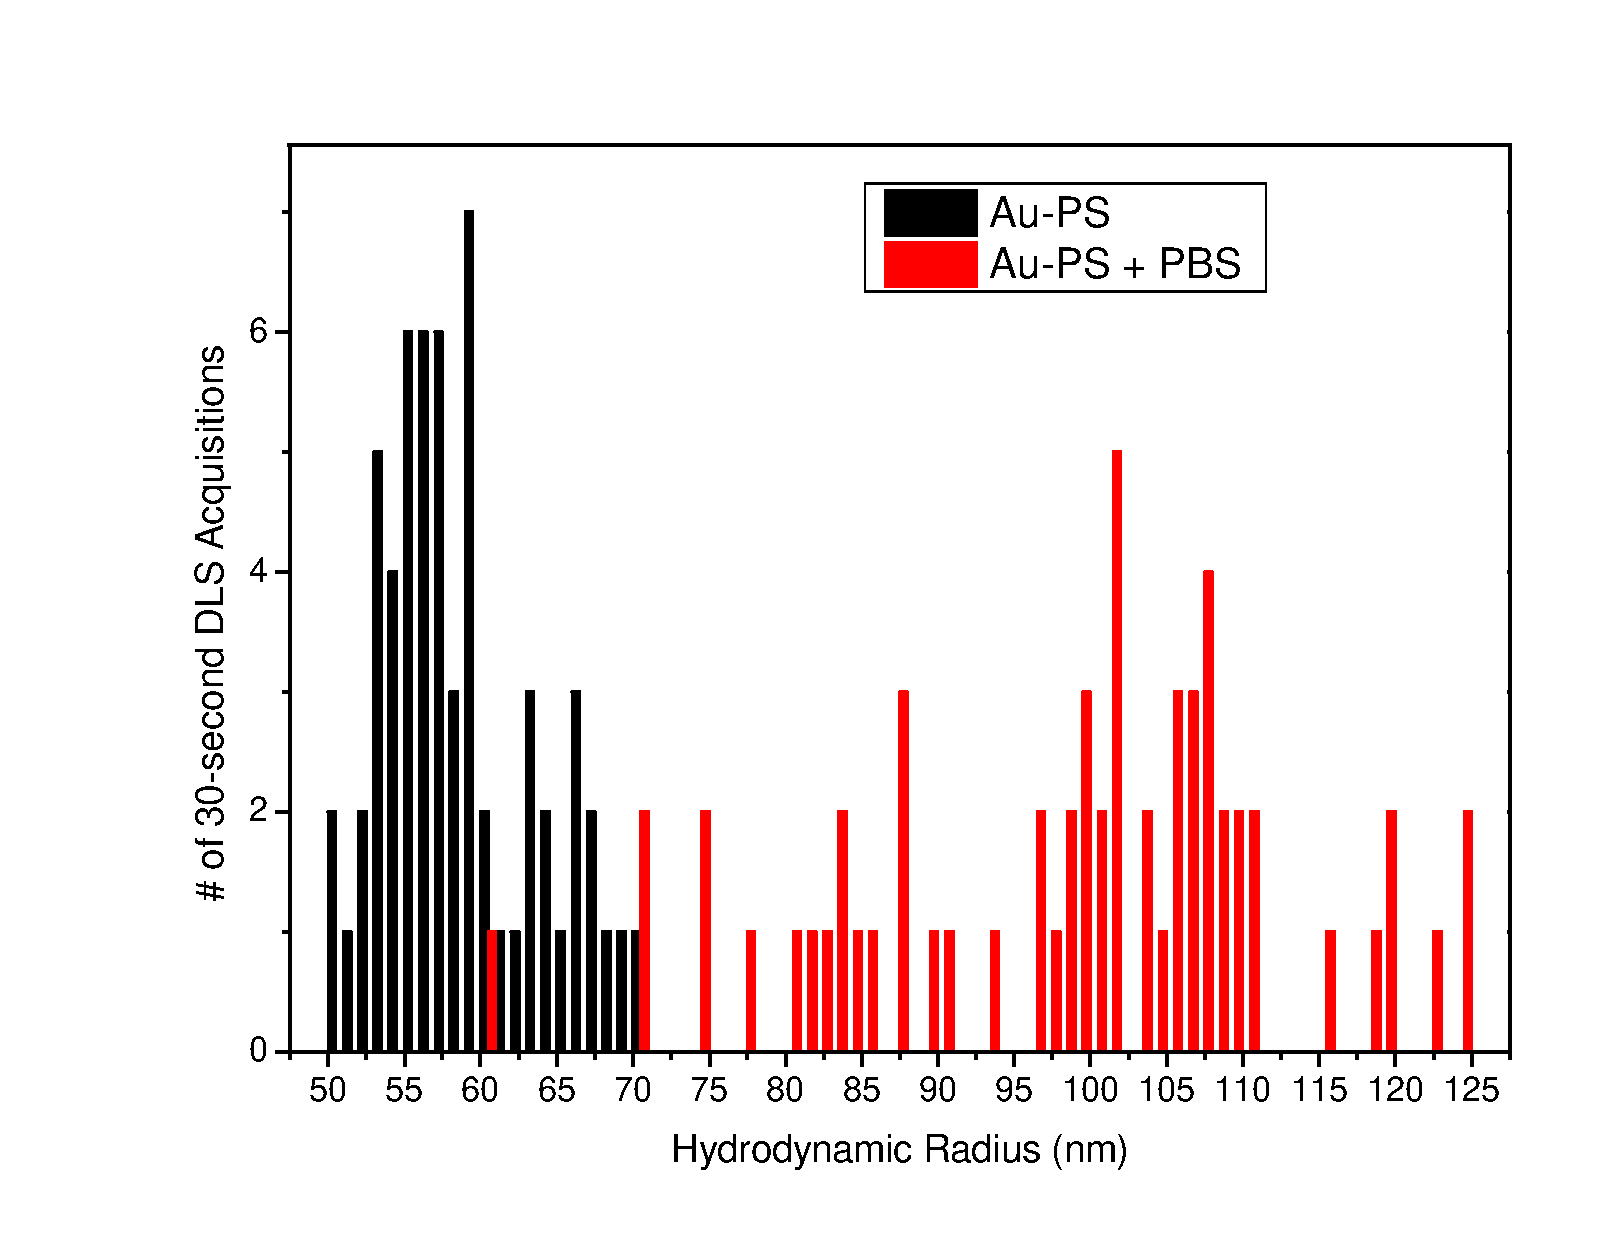
\includegraphics[keepaspectratio,width=4in,height=0.75\textheight]{10^7.pdf}
\caption{Histogram of radii of 30-second DLS acquisitions of $10^7$ 1 kDa PS/Au with and without PBS from the summer of 2010. The distribution is noticeably shifted to the right and flattened after the addition of PBS. Data taken by Ellis and Hoidn~\citep{hoidnellis}.}
\label{protection1kda}
\end{figure}



At the end of the summer of 2010, 5 kDa PEG-SH had not yet been used or characterized, so a completely new optimization process had to be a applied. This consisted of measuring the radii of the gold spheres immediately after the addition of a variety of concentrations of 5 kDa PEG-SH (\autoref{titrationstudy}); measuring the radii of the same solutions after an incubation period (\autoref{timestudy}); and measuring the radii of some solutions after addition of salt solution (\autoref{protectionstudy}). These measurements yielded a monolayer number for 5 kDa PEG-SH of approximately 50,000 PS\slash Au. Strong protection of the nanospheres was also demonstrated at 10,000 PS\slash Au. Therefore, 10,000 PS\slash Au was used as the concentration for the full protocol, as it provides protection, and there should already be a monolayer of OPAb on the surface of the nanospheres.

\section{Titration Study}
\label{titrationstudy}

A titration curve was made by adding 5 kDa PS to 90 nm gold nanospheres (R=52 nm) in varying concentrations, from 1000 PS per nanosphere to $10^7$ PS per nanosphere; the broad range was used to determine the range of concentrations in which the monolayer formed. The hydrodynamic radii of these PEGylated nanospheres were then measured using the Dynamic Light Scattering (DLS) instrument, taking 15 30-second acquisitions of each solution and discarding the first three to account for temperature acclimation. The results of these exploratory measurements are shown in \autoref{kdapegshnewexpl}.

\begin{figure}[htbp]
\centering
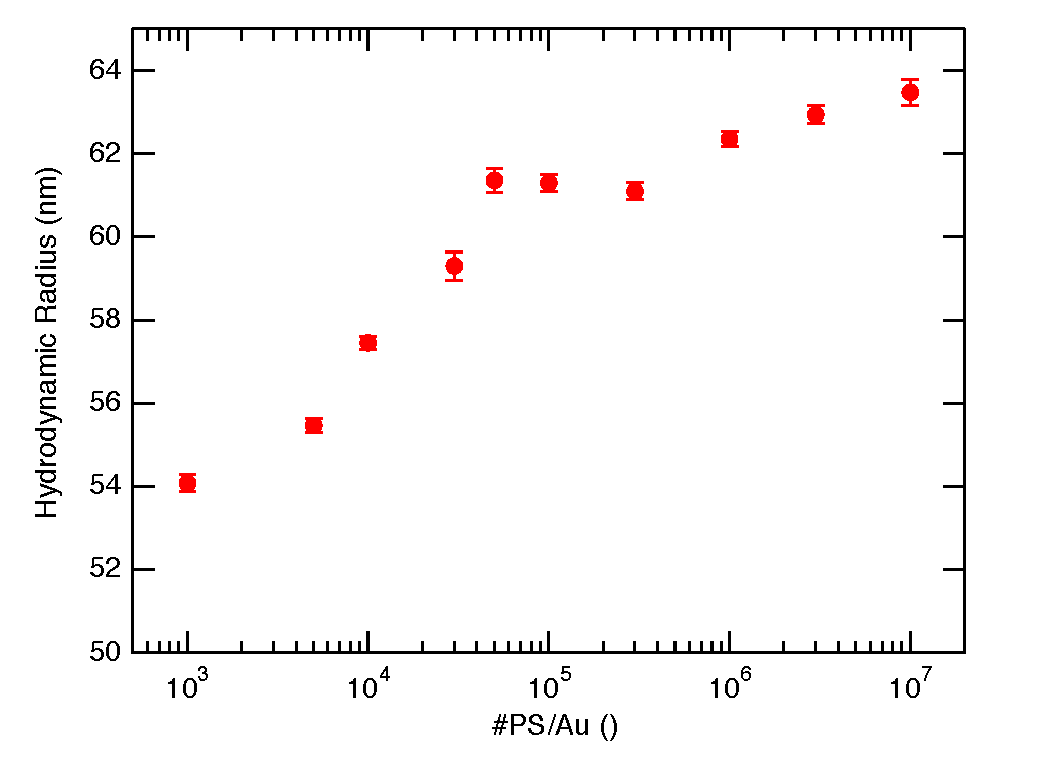
\includegraphics[keepaspectratio,width=\textwidth,height=0.75\textheight]{./ImmediateExploratory.pdf}
\caption{Plot of hydrodynamic radii of Au nanospheres from 1,000 to $10^7$ PS\slash Au less than 30 minutes after addition of PS.}
\label{kdapegshnewexpl}
\end{figure}



This plot shows the behavior of a rapid rise followed by a plateau that is expected of a species forming a monolayer on a surface. The plateau begins to appear around 100,000 \#PS\slash Au, so two more measurements were taken with a spread of concentrations around that range. A plot of the averages of the radii of the repeated concentrations are shown in \autoref{kdapegshnewavg}. This data suggests that the monolayer is formed at approximately 50,000 \#PS\slash Au, with a radius of $60.4\pm0.3$ nm.

\begin{figure}[htbp]
\centering
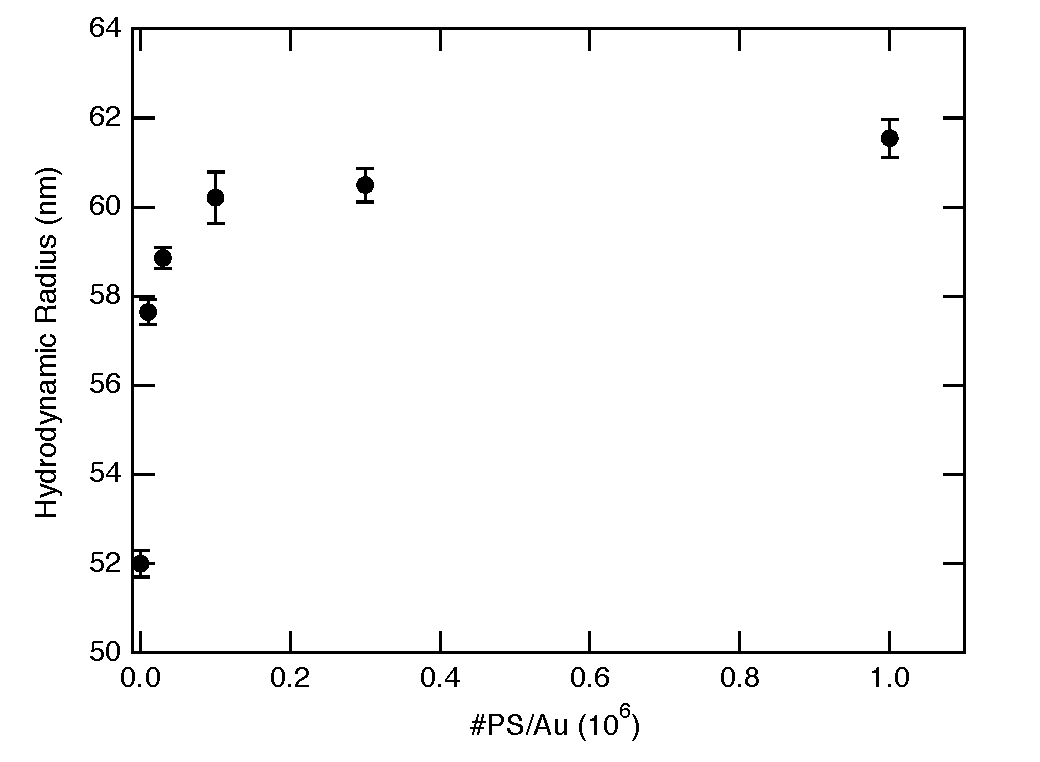
\includegraphics[keepaspectratio,width=\textwidth,height=0.75\textheight]{ImmediateAvg.pdf}
\caption{Plot of hydrodynamic radii of Au nanospheres at 10,000, 30,000, 100,000, 300,000, and $10^6$ PS\slash Au less than 30 minutes after addition of PS. Points are formed by taking the mean and standard error of three independent measurements at each concentration.}
\label{kdapegshnewavg}
\end{figure}



\section{Time Study}
\label{timestudy}

The same samples used in the titration study were measured again after 48--72 hours of incubation, producing the radii shown in \autoref{kdapegshtime}.

\begin{figure}[htbp]
\centering
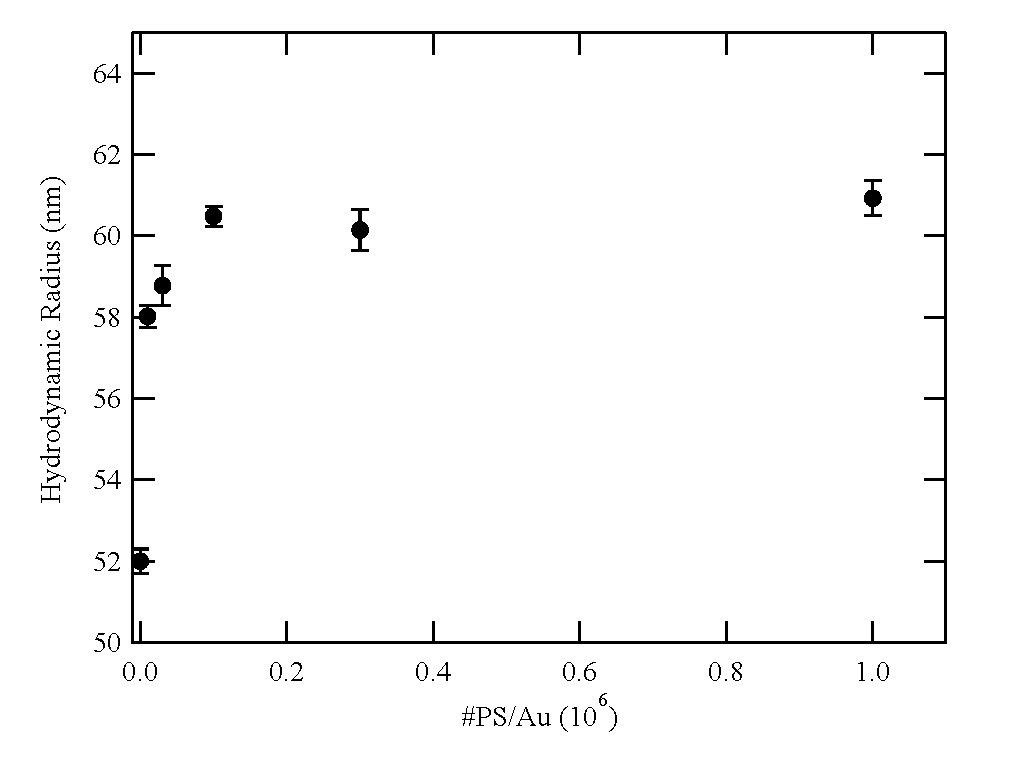
\includegraphics[keepaspectratio,width=\textwidth,height=0.75\textheight]{TimeAvg.pdf}
\caption{Plot of hydrodynamic radius of Au nanospheres at the same concentrations as in \autoref{kdapegshnewavg} 48--72 hours after addition of PS. Points are formed by taking the mean and standard error of three independent measurements at each concentration.}
\label{kdapegshtime}
\end{figure}



The plateau in this graph is slightly sharper than in \autoref{kdapegshnewavg}, indicating that van der Waals forces and thiol bonding processes are in competition, with van der Waals binding dominating immediately after addition, but the lower-energy thiol bonds dominating after incubation time. This leads to the increased radius of the lower-radius samples and the decreased radius of the higher-radius samples. However, the plateau region still has $R=60.3\pm0.3$ nm, as a second indication of a monolayer. Clearly, it is essential that PEG-SH be allowed to incubate with spheres to allow for the PEG-SH binding to reach equilibrium.

More information about the final monolayer state can be gained from determining the apparent number of PEG-SH molecules bound to the nanosphere. A single 5 kDa PEG-SH molecule, with a density of $1.11\,\mathrm{\frac{g}{cm^3}}$, has a volume of
\[\mathrm{V_{5\,kDa\ PEG-SH}}
=\frac{5\mathrm{kDa}}{1.11\frac{\mathrm g}{\mathrm cm^3}}=7.5\mathrm{\,nm^3}\]
This means that a 5 kDa PEG-SH monolayer has, based on the change in hydrodynamic radius,
\[\#_{\mathrm{5\,kDa\ PEG-SH}}=
\frac{\frac{4}{3}\pi((60.5\mathrm{\,nm})^3-(51.0\mathrm{\,nm})^3)} {V_{\mathrm{5\,kDa\ PEG-SH}}}=48,400\pm900\mathrm{\ 5\,kDa\ PEG-SH}\]
This indicates that the measurement of the plateau as beginning at 50,000 PEG-SH per nanosphere is correct. This also allows us to get a sense of the effective footprint of a PEG-SH molecule as it sits on the gold. At monolayer concentration, the area on the surface of the gold taken up by each PEG-SH molecules is
\[A_{\mathrm{PS}}=\frac{4\pi(51.5\mathrm{\,nm})^2/\mathrm{Au}} {47,500\,\mathrm{\frac{PS}{Au}}}=0.70\pm0.03\frac{\mathrm{nm}^2}{\mathrm{PS}}=70\pm3\frac{\text{\AA}^2}{\mathrm{PS}}\]
This size is determined partially by the atomic size of the sulfur atom ($D=2\text{\AA}$), but mostly by the extent to which the PEG chain is bunched; clearly, most of the effective width comes from the bunching.

\section{Protection Study}
\label{protectionstudy}

As mentioned above, the main reason for using 5 kDa PEG-SH is to prevent the Au nanospheres from agglomerating. The Au nanosphere solution includes a negatively charged capping agent that makes the spheres repel each other; when the solution is buffered at pH \ensuremath{\sim}7.5 to prevent antibodies from denaturing during the full immunogold procedure, positive ions are introduced into the solution that neutralize the capping agents, causing the gold nanospheres to agglomerate. Theoretically, PEG-SH would prevent this from happening, but 1 kDa PEG-SH does not, as shown in \autoref{protection1kda}.

Therefore, the protection capabilities of 5 kDa PS were tested by adding PEG-SH to the Au nanospheres in various concentrations, then mixing those solutions in equal volumes with commercial PBS, which has a salt concentration of approximate 150 mM. The spheres were allowed to incubate for at least 30 minutes with the PBS, then measured in the DLS. Selected results from those measurements are shown in \autoref{protection}.

\begin{figure}[htbp]
\centering
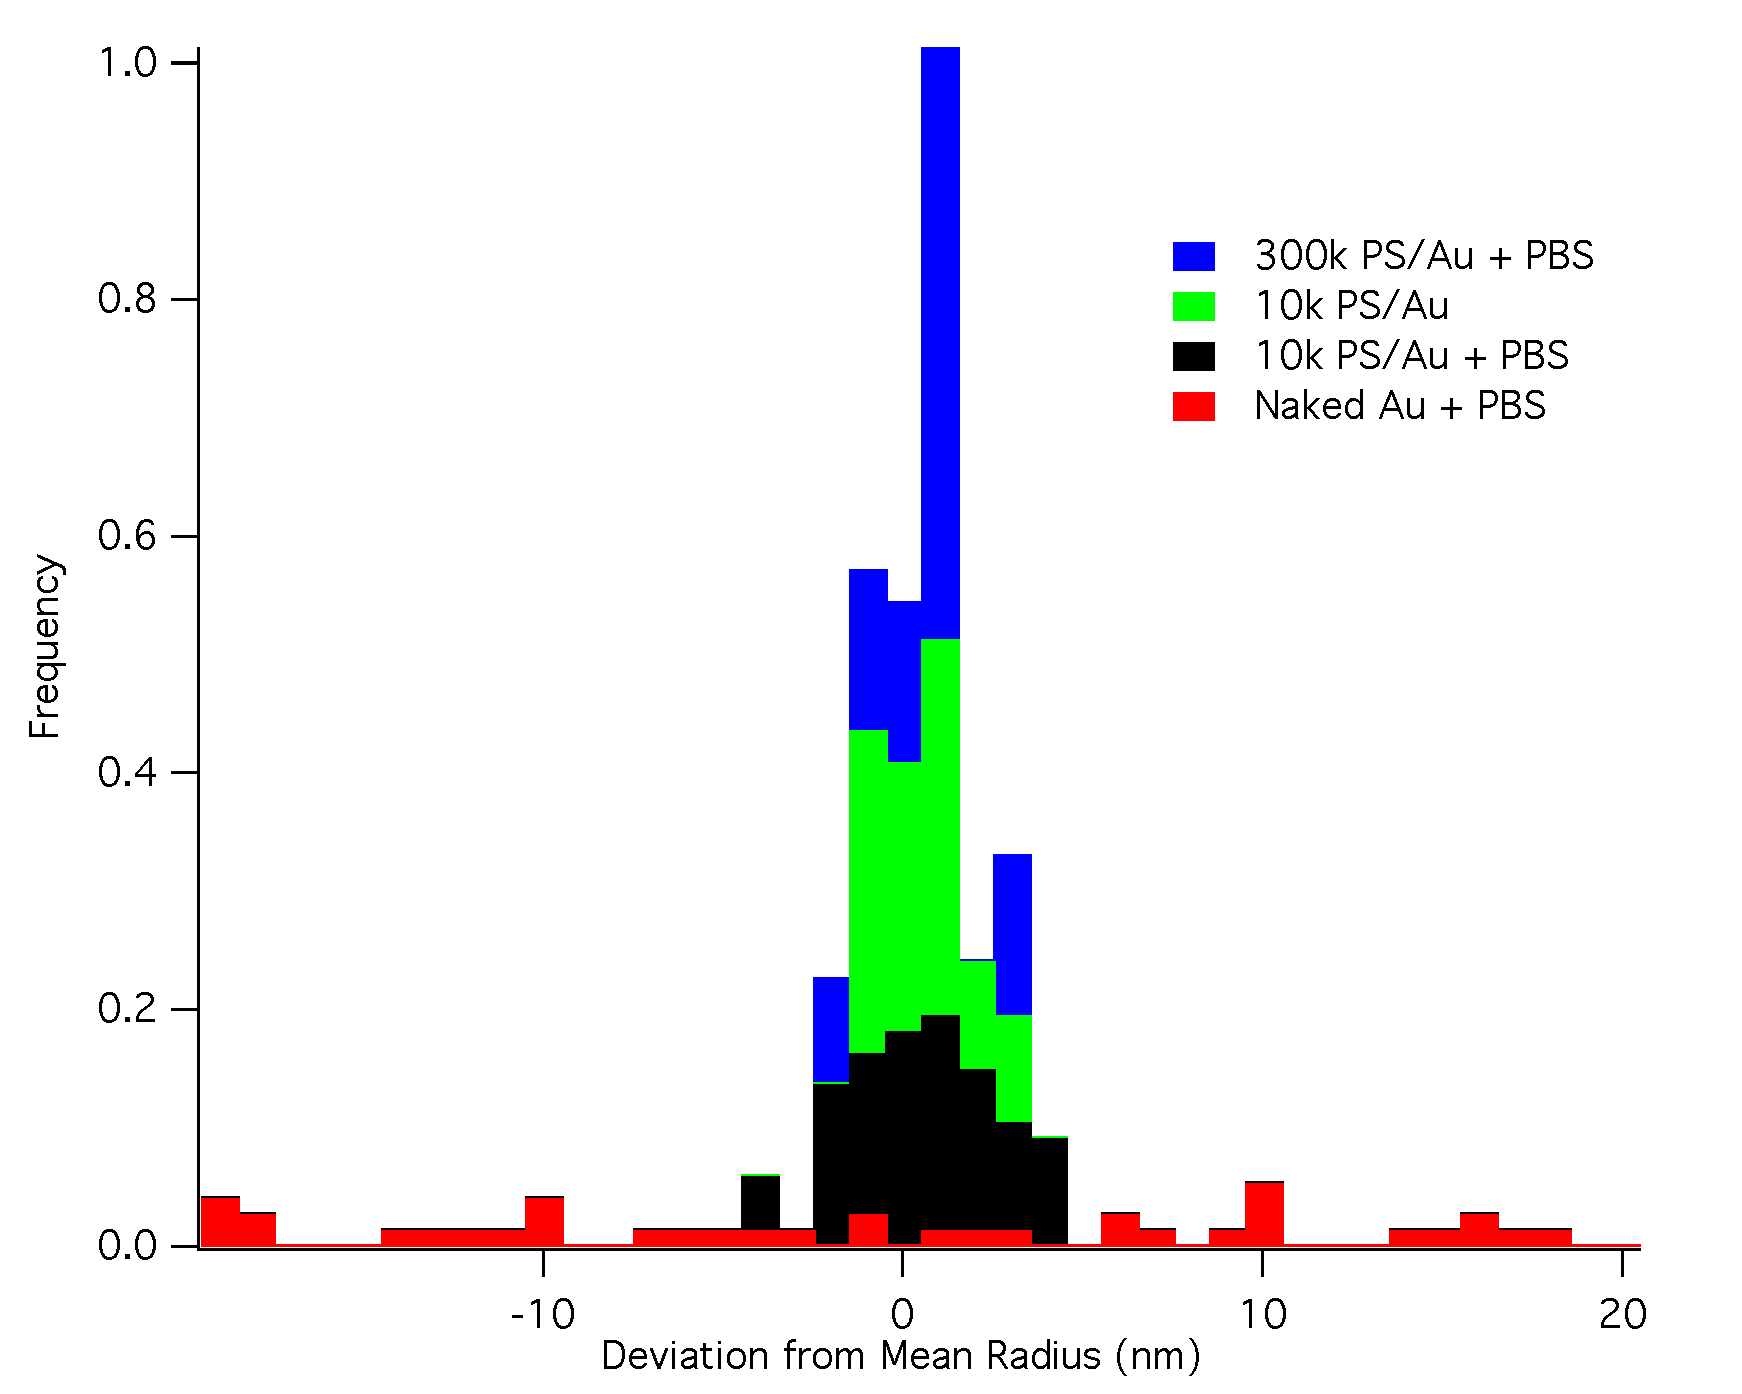
\includegraphics[keepaspectratio,width=5in,height=0.75\textheight]{RadiusHistPBS.pdf}
\caption{Stacked histograms of differing concentrations of Au-PS with and without PBS. The naked gold is significantly broader than any of the other distributions.}
\label{protection}
\end{figure}



For all but the naked gold, almost all acquisitions are within 3 nm of the mean; this is also true of the 300k PS\slash Au without PBS from the summer of 2010. However, with just 10k 5 kDa PS\slash Au, the width of the distribution barely widens when PBS is added--a stark contrast to the addition of PBS to 300k 1 kDa PS\slash Au. Furthermore, there was a \ensuremath{\sim}15 nm increase in average radius between the 1 kDa PS spheres with and without PBS. In the case of the 10k 5 kDa PS\slash Au, the difference in average radius was negligible: 0.09 nm.

From observing the lack of change in both average radius and the change in radial distribution when using the 5 kDa PEG-SH, it is clear that the 5 kDa PEG-SH fully protects the Au nanospheres against capping agent neutralization. There is, however, a noticeable difference between the 10k and 300k PS\slash Au samples; the 300k is slightly narrower, indicating that it offers slightly more protection, consistent with the 300k PS\slash Au solution being on the plateau while the 10k PS\slash Au is still on the rising part of the titration curve.